\section{App}

\begin{figure}[h]
	\centering
	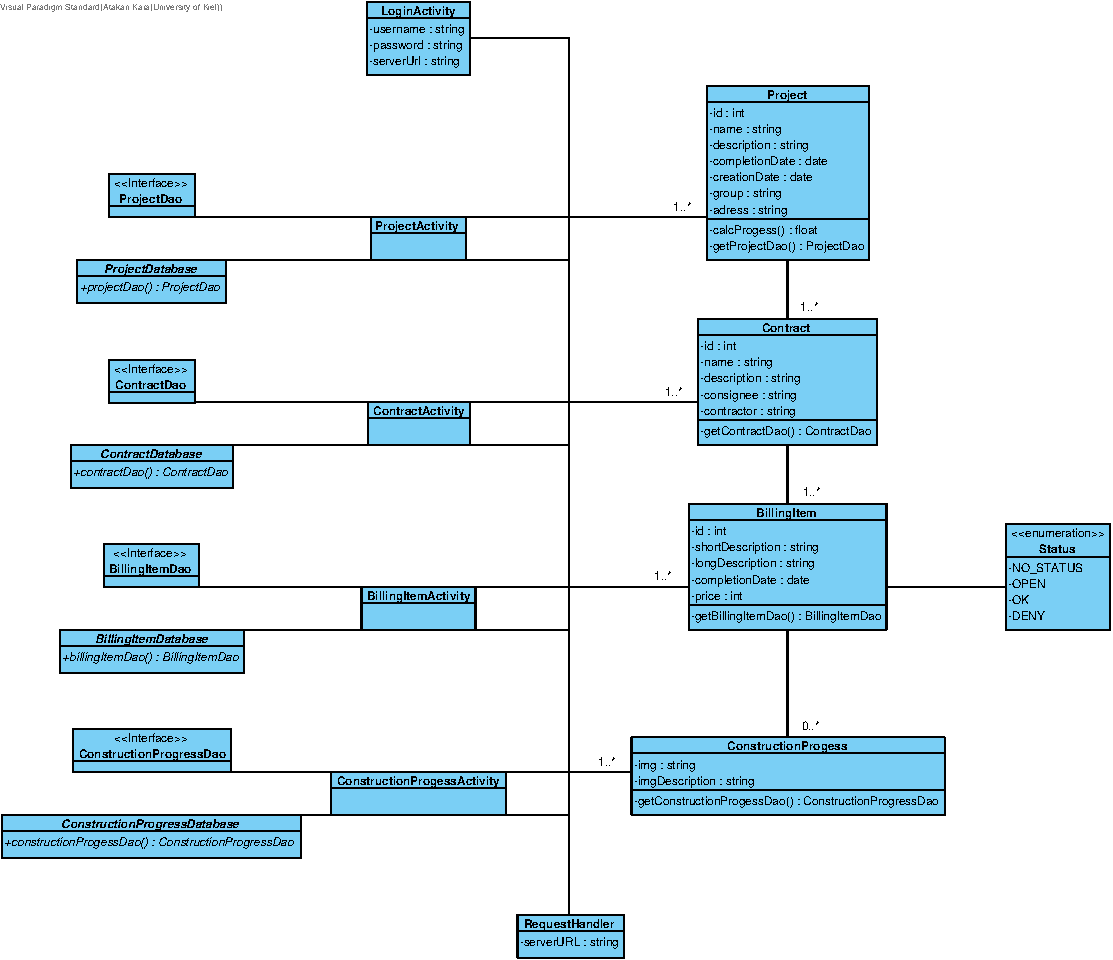
\includegraphics[width=16cm]{img/diagrams/Classdiagram-App.pdf}
	\caption{Klassendiagramm - App}
	\label{fig:klassendiagramm-a}
\end{figure}

\clearpage

\begin{table}[h]
	\centering
	\begin{tabularx}{\textwidth}{X X}
		\rowcolor[HTML]{C0C0C0} 
		\textbf{Klassenname} & \textbf{Aufgabe} \\
		Project & Bauplan eines Projektes mit den jeweiligen Attributen.\\
		\rowcolor[HTML]{E7E7E7} 
		Contract & Bauplan eines Vertrages mit den jeweiligen Attributen. \\
		BillingItem & Bauplan einer Leistungsposition mit den jeweiligen Attributen. \\
		\rowcolor[HTML]{E7E7E7} 
		ConstructionProgress & Bauplan einer Baufortschritts-Klasse mit den jeweiligen Attributen. \\
		LoginActivity & Verwaltung des Login-Bildschirms. \\
		\rowcolor[HTML]{E7E7E7} 
		ProjectActivity & Verwaltung des Projekt-Bildschirms. \\
		ContractActivity & Verwaltung des Vertags-Bildschirms. \\
		\rowcolor[HTML]{E7E7E7} 
		BillingItem & Verwaltung des Leistungspositions-Bildschirms. \\
		ConstructionProgressActivity & Verwaltung des Baufortschritts-Bildschirms. \\
		\rowcolor[HTML]{E7E7E7} 
		RequestHandler & Verwaltung der Netzwerkanfragen aller Klassen. \\
		ProjectDao & Datenzugriffsobjekt mit Anfragen zur Interaktion mit der Projektdatenbank. \\
		\rowcolor[HTML]{E7E7E7} 
		ProjectDatabase & Room-Datenbank für Projekte. \\
		ContractDao & Datenzugriffsobjekt mit Anfragen zur Interaktion mit der Vertragsdatenbank. \\
		\rowcolor[HTML]{E7E7E7} 
		ContractDatabase & Room-Datenbank für Verträge. \\
		BillingItemDao & Datenzugriffsobjekt mit Anfragen zur Interaktion mit der Leistungspositionsdatenbank. \\
		\rowcolor[HTML]{E7E7E7} 
		BillingItemDatabase & Room-Datenbank für Leistungspositionen. \\
		ConstructionProgressDao & Datenzugriffsobjekt mit Anfragen zur Interaktion mit der Baufortschritsdatenbank. \\
		\rowcolor[HTML]{E7E7E7} 
		ConstructionProgressDatabase & Room-Datenbank für den Baufortschritt. \\
		Status & Enumeration des Typs Status.
	\end{tabularx}
	\caption{Klassenbeschreibung - App}
	\label{table:klassenbeschreibung-a}
\end{table}